\newpage
\subsubsection{KP03. Manajemen Barang Lelang}
\label{kp03}
Pada kasus penggunaan ini, pengguna akan dapat memanajemen barang yang ia daftarkan untuk dilelang, dan melihat proses monitoringnya, seperti yang dipaparkan pada penjelasan berikut.\\

\begin{figure}[H]
	\centering
	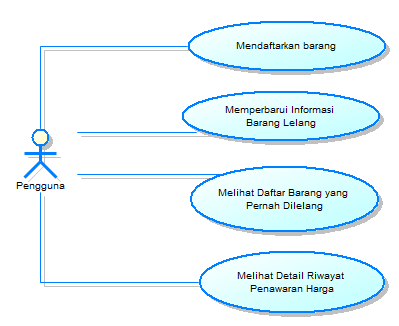
\includegraphics
	[width=\textwidth]
	{images/bab3/usecasediagram/ucd-03.png}
	\caption{Diagram Kasus Penggunaan Manajemen Barang Lelang}
	\label{ucd.03}
\end{figure}
\newpage
% Mendaftarkan barang untuk dilelang
% Mendaftarkan barang untuk dilelang

\begin{table}[H]
	\centering
\begin{tabular}{|r|p{8cm}|}
		\hline
		\textbf{Kode}                                                    & UC-01.01                                                     \\ \hline
		\textbf{Nama}                                                    & \textbf{Mendaftarkan Barang Lelang}                                         \\ \hline
		\textbf{Aktor}                                                   & Pengguna                                                    \\ \hline
		\textbf{Deskripsi}                                               & Pengguna mendaftarkan barang untuk dilelang di dalam sistem \\ \hline
		\textbf{Tipe}                                                    & Fungsional                                                  \\ \hline
		\textbf{\textit{Precondition}}
			& Barang yang akan dilelang belum terdaftar dalam sistem \\ \hline
		\textbf{\textit{Postcondition}} 
			& Barang yang akan dilelang sudah terdaftar dalam sistem \\ \hline
		\multicolumn{2}{|c|}{\textbf{Alur Kejadian Normal}}                                                                            \\ \hline
		\multicolumn{1}{|l|}{}                                           & 
			\begin{enumerate}
				\item Pengguna membuka Halaman Registrasi
				\item \label{uc0101-show1page}Sistem menampilkan halaman yang berisi Form Registrasi
				\item Pengugna mengisi form tersebut
				\item Setelah selesai mengisi, pengugna mengklik tombol "Registrasi"
				\item \label{al-0101-a} Sistem memvalidasi data yang dimasukkan pengguna
				\item Jika data valid, sistem me\textit{redirect} ke halaman \textit{landing page} dalam keadaan sudah terautentikasi \& aun berhasil didaftarkan.
			\end{enumerate}
		\\ \hline
		\multicolumn{2}{|c|}{\textbf{Alur Kejadian Alternatif}}                                                         \\ \hline
		\multicolumn{1}{|l|}{}                                           & \textbf{Data yang dimasukkan pengguna tidak valid}
			\\ \hline
		\multicolumn{1}{|l|}{}                                           & 
			 \begin{itemize}
			 	\item[\ref{al-0101-a}a.] Sistem tidak dapat memvalidasi data yang dimasukkan pengguna.
			 	\item[\ref{al-0101-a}b.] Sistem me\textit{redirect} ke halaman form registrasi (langkah \ref{uc0101-show1page}) dengan \textit{error message}.
			 \end{itemize}
		 \\ \hline
	\end{tabular}
	\caption{Spesifikasi Kasus Penggunaan Registrasi }
	\label{uc01.01}
\end{table}

% Memperbarui informasi barang yang dilelang
% Memperbarui informasi barang yang dilelang

\begin{table}[H]
	\centering
	\begin{tabular}{|r|p{8cm}|}
		\hline
		\textbf{Kode}                                                    & UC-03.02                                                     \\ \hline
		\textbf{Nama}                                                    & \textbf{Memperbarui informasi barang yang dilelang} \\ \hline
		\textbf{Aktor}                                                   & Pengguna 
			\\ \hline
		\textbf{Deskripsi}                                               & Pengguna memperbarui informasi barang yang sebelumnya sudah terdaftar di dalam sistem 
			 \\ \hline
		\textbf{Tipe}                                                    & Fungsional 
			\\ \hline
		\textbf{\textit{Precondition}}
			& Informasi barang belum diperbarui. \\ \hline
		\textbf{\textit{Postcondition}} 
			& Informasi barang sudah diperbarui. \\ \hline
		\multicolumn{2}{|c|}
			{\textbf{Alur Kejadian Normal}}                                                                            \\ \hline
		\multicolumn{1}{|l|}{}                                           & 
			\begin{enumerate}
				\item Pengguna dalam keadaan terautentikasi, mengklik "Item Anda" -> "Manage Items" pada \textit{navbar} bagian atas halaman.
				\item \label{uc0302-show1page}Sistem menampilkan halaman yang berisi daftar barang yang didaftarkan pengguna.
				\item Pengguna mengklik barang yang ingin diperbarui informasinya
				\item \label{uc0302-show2page}Sistem menampilkan halaman \textit{form} "Perbarui barang".
				\item Pengguna mengisi informasi pembaruan barang di dalam form tersebut.
				\item Setelah selesai, pengguna mengklik tombol "Simpan Pembaruan".
				\item \label{al-0302-a} Sistem memvalidasi data (termasuk file gambar) yang dimasukkan pengguna
				\item Jika data valid, sistem me\textit{redirect} ke halaman "Kelola Barang" dalam keadaan barang baru sudah ditambahkan.
			\end{enumerate}
		\\ \hline
		
		\multicolumn{2}{|c|}{\textbf{Alur Kejadian Alternatif}}                                                         \\ \hline
		\multicolumn{1}{|l|}{}                                           & \textbf{Data barang yang dimasukkan pengguna tidak valid}
			\\ \hline
		\multicolumn{1}{|l|}{}                                           & 
			 \begin{itemize}
			 	\item[\ref{al-0302-a}a.] Sistem tidak dapat memvalidasi data yang dimasukkan pengguna.
			 	\item[\ref{al-0302-a}b.] Sistem me\textit{redirect} ke halaman "Perbarui Barang" (langkah \ref{uc0302-show2page}) dengan \textit{error message}.
			 \end{itemize}
		 \\ \hline
		 \multicolumn{1}{|l|}{}                                           & \textbf{Gambar yang dimasukkan pengguna tidak dapat divalidasi}
		 \\ \hline
		 \multicolumn{1}{|l|}{}                                           & 
		 \begin{itemize}
		 	\item[\ref{al-0302-a}a.] Sistem menampilkan \textit{error modal} berisi peringatan bahwa "Kesalahan saat \textit{upload} gambar, silahkan coba lagi"
		 	\item[\ref{al-0302-a}b.] Sistem me\textit{redirect} ke halaman form "Perbarui Barang" (langkah \ref{uc0301-show2page}) dengan \textit{error message}.
		 \end{itemize}
		 \\ \hline
	\end{tabular}
	\caption{Spesifikasi Kasus Penggunaan : Mendaftarkan Barang Lelang}
	\label{uc03.02}
\end{table}

% Melihat barang yang pernah didaftarkan
% Melihat barang yang pernah didaftarkan

\begin{table}[H]
	\centering
	\begin{tabular}{|r|p{8cm}|}
		\hline
		\textbf{Kode}                                                    & UC-03.03                                                     \\ \hline
		\textbf{Nama}                                                    & \textbf{Melihat Daftar Barang yang Pernah Dilelang} \\ \hline
		\textbf{Aktor}                                                   & Pengguna 
		\\ \hline
		\textbf{Deskripsi}                                               & Pengguna hendak melihat daftar semua barang yang pernah didaftarkan untuk dilelang di dalam sistem.
		\\ \hline
		\textbf{Tipe}                                                    & Fungsional 
		\\ \hline
		\textbf{\textit{Precondition}}
		& Informasi daftar barang belum ditampilkan. \\ \hline
		\textbf{\textit{Postcondition}} 
		& Informasi daftar barang sudah ditampilkan. \\ \hline
		\multicolumn{2}{|c|}
		{\textbf{Alur Kejadian Normal}}                                                                            \\ \hline
		\multicolumn{1}{|l|}{}                                           & 
		\begin{enumerate}
			\item Pengguna dalam keadaan terautentikasi, mengklik "Item Anda" -> "Manage Items" pada \textit{navbar} bagian atas halaman.
			\item \label{uc0302-show1page}Sistem menampilkan halaman yang berisi daftar barang yang didaftarkan pengguna.
		\end{enumerate}
		\\ \hline
		\multicolumn{2}{|c|}{\textbf{Alur Kejadian Alternatif}}                                                         \\ \hline
		\multicolumn{1}{|l|}{}                                           & -
		\\ \hline
	\end{tabular}
	\caption{Spesifikasi Kasus Penggunaan : Melihat Barang yang Pernah Didaftarkan}
	\label{uc03.03}
\end{table}

% Melihat riwayat harga yang ditawarkan pada barang yang dilelang
% Melihat riwayat harga yang ditawarkan pada barang yang dilelang

\begin{table}[H]
	\centering
	\begin{tabular}{|r|p{8cm}|}
		\hline
		\textbf{Kode}                                                    & UC-03.04                                                     \\ \hline
		\textbf{Nama}                                                    & \textbf{Melihat Detail Riwayat Penawaran Harga} \\ \hline
		\textbf{Aktor}                                                   & Pengguna 
		\\ \hline
		\textbf{Deskripsi}                                               & Pengguna hendak melihat daftar semua barang yang pernah didaftarkan dalam sistem.
		\\ \hline
		\textbf{Tipe}                                                    & Fungsional 
		\\ \hline
		\textbf{\textit{Precondition}}
		& Informasi daftar barang belum ditampilkan. \\ \hline
		\textbf{\textit{Postcondition}} 
		& Informasi daftar barang sudah ditampilkan. \\ \hline
		\multicolumn{2}{|c|}
		{\textbf{Alur Kejadian Normal}}                                                                            \\ \hline
		\multicolumn{1}{|l|}{}                                           & 
		\begin{enumerate}
			\item Pengguna dalam keadaan terautentikasi, mengklik "Item Anda" -> "Manage Items" pada \textit{navbar} bagian atas halaman.
			\item Sistem menampilkan halaman yang berisi daftar barang yang didaftarkan pengguna.
			\item Pengguna mengklik barang yang ingin dilihat daftar penawaran harganya
			\item Sistem menampilkan halaman detail informasi barang
			\item Pengguna mengklik tombol "Lihat Riwayat Penawaran"
			\item Sistem menampilkan halaman berisi daftar riwayat penawaran.
		\end{enumerate}
		\\ \hline
		\multicolumn{2}{|c|}{\textbf{Alur Kejadian Alternatif}}                                                         \\ \hline
		\multicolumn{1}{|l|}{}                                           & -
		\\ \hline
	\end{tabular}
	\caption{Spesifikasi Kasus Penggunaan : Melihat Riwayat Penawaran Harga}
	\label{uc03.04}
\end{table}